\chapter{Лабораторная работа 3 \\
Имитационное моделирование RF-моделей}

Цель работы: научиться проводить имитационное моделирование ВЧ-цепей, получить навыки работы со средой моделирования Advanced Design System (ADS).

\section{Техническое задание}

Спроектировать приёмный канал приёмо-передающего модуля общего назначения.
Параметры МШУ: $K_p = 13~\text{дБ}$, $K_\text{ш} = 2.3~\text{дБ}$, $TOI = 38~\text{дБм}$, $P1dB = 22~\text{дБм}$.
Параметры УМ: $K_p = 21.5~\text{дБ}$, $K_\text{ш} = 2.5~\text{дБ}$, $TOI = 41~\text{дБм}$, $P1dB = 21~\text{дБм}$.
Частотные параметры: $f_{RF} = 3~\text{ГГц}$, $f_{IF} = 150~\text{МГц}$, $\Delta f_{-3dB} = 84~\text{МГц}$.

\section{Выполнение работы}

\subsection{Расчёт системы методом гармонического баланса}

Соберём моделируемую схему (Рис.~\ref{fig:simulation_modeling_schematic_1}) и запустим моделирование.
Выведем гармоники до и после смесителя (Рис.~\ref{fig:simulation_modeling_data_1}).

\begin{figure}[!ht]
    \centering
    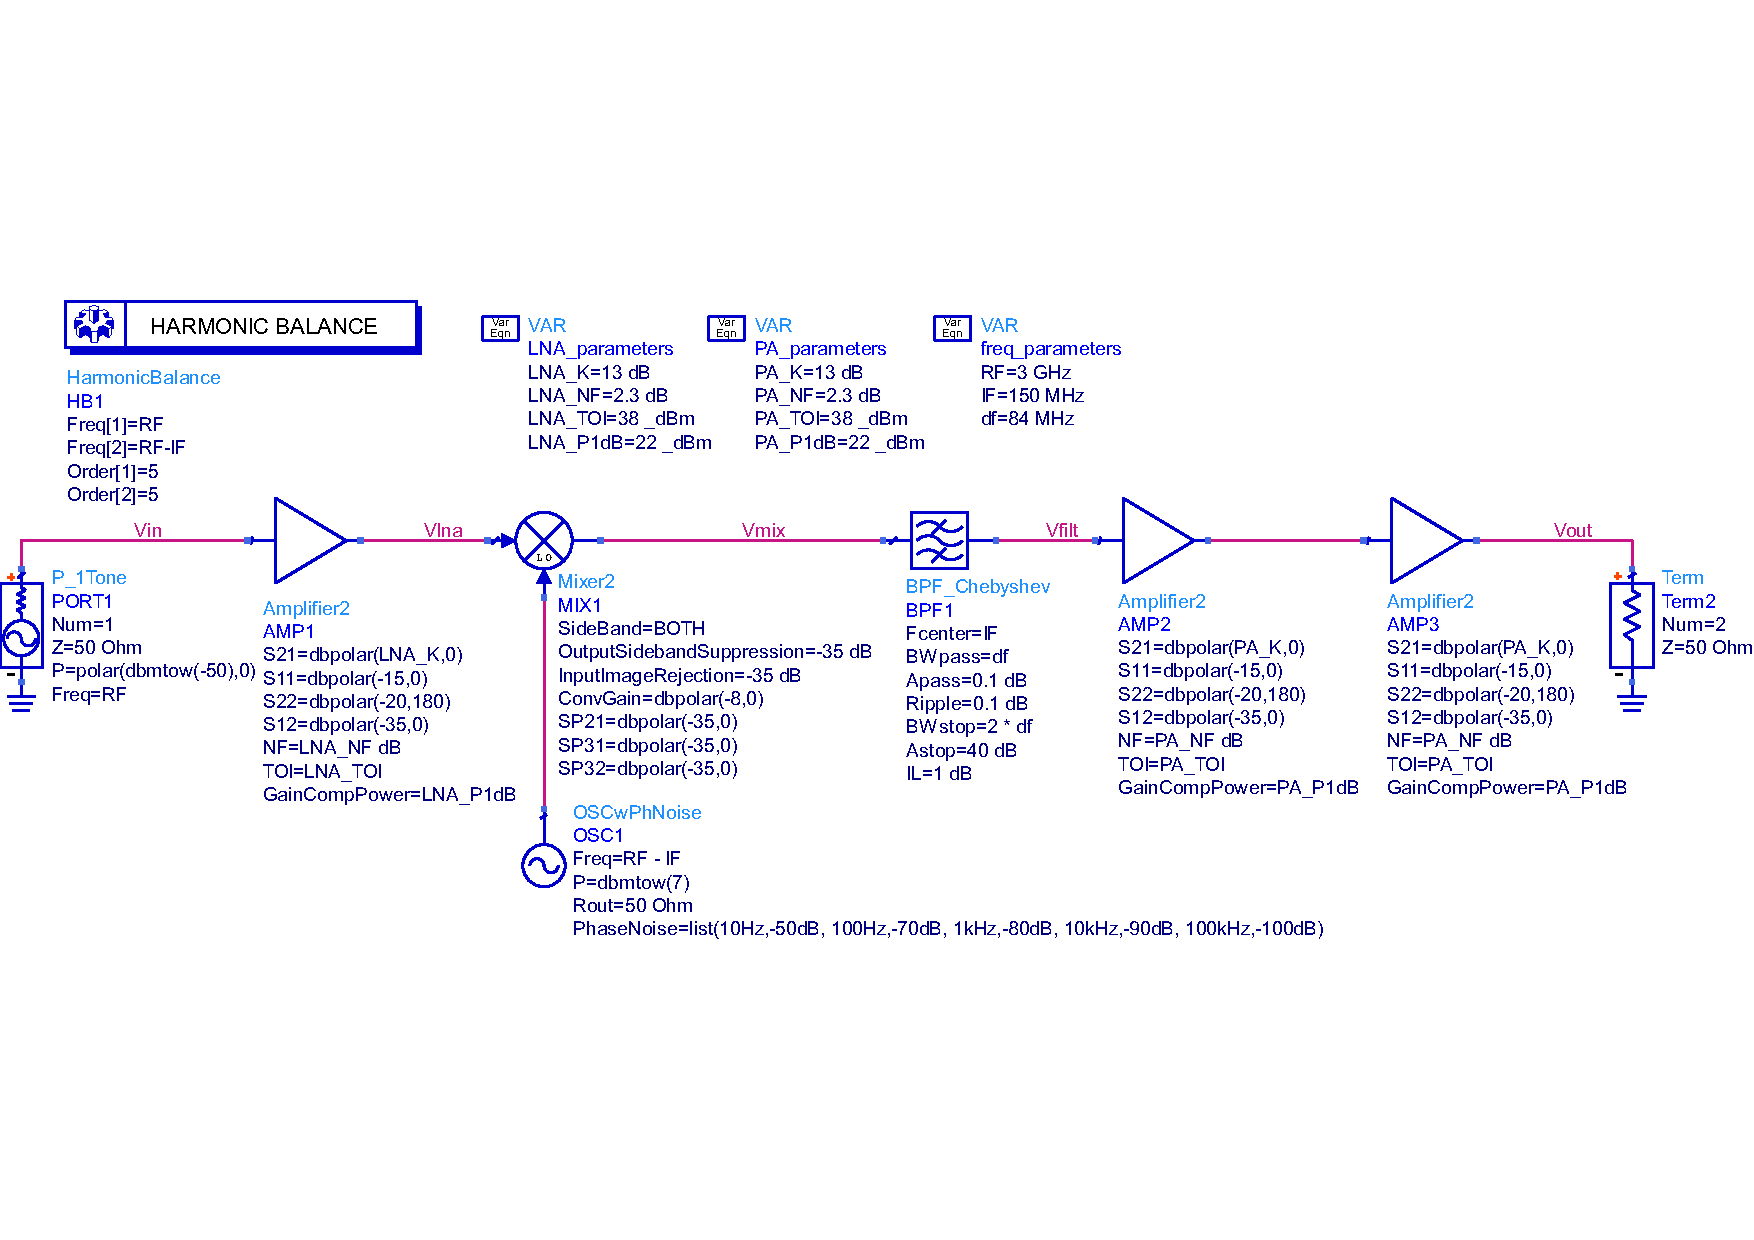
\includegraphics[width=0.7\textwidth]{simulation_modeling_schematic_1.pdf}
    \caption{Моделируемая схема}%
    \label{fig:simulation_modeling_schematic_1}
\end{figure}

\begin{figure}[!ht]
    \centering
    \begin{subfigure}[b]{0.7\textwidth}
        \centering
        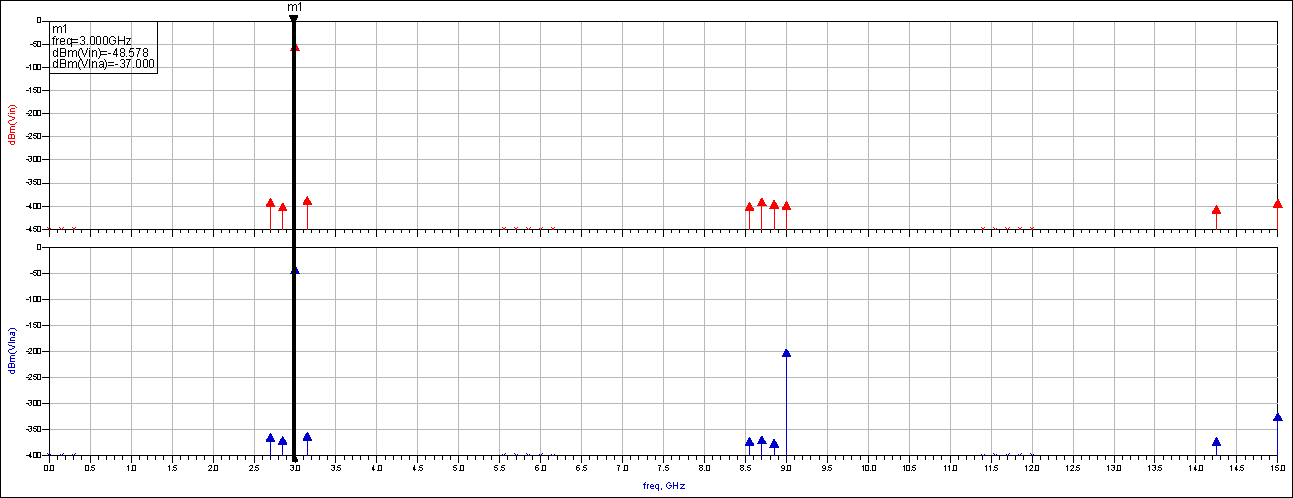
\includegraphics[width=\textwidth]{simulation_modeling_data_1_harmonics_before_mixer.pdf}
        \caption{}%
        \label{fig:simulation_modeling_data_1_harmonics_before_mixer}
    \end{subfigure}
    \vfill
    \begin{subfigure}[b]{0.7\textwidth}
        \centering
        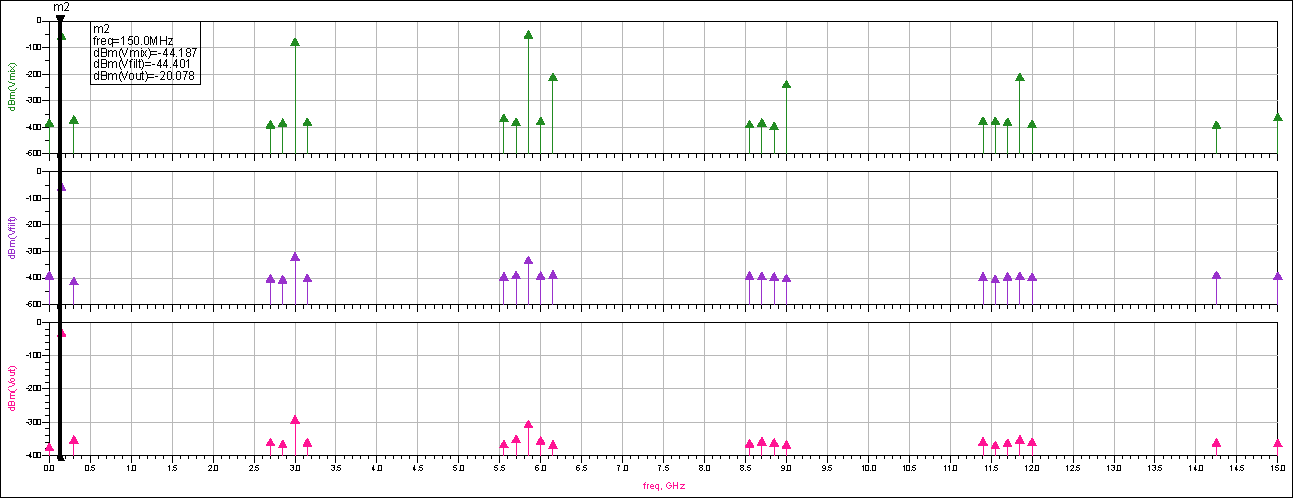
\includegraphics[width=\textwidth]{simulation_modeling_data_1_harmonics_after_mixer.pdf}
        \caption{}%
        \label{fig:simulation_modeling_data_1_harmonics_after_mixer}
    \end{subfigure}
        \caption{%
            (а) Гармоники до смесителя;
            (б) гармоники после смесителя
        }%
        \label{fig:simulation_modeling_data_1}
\end{figure}

\subsection{Определение точки 1~дБ компрессии}

Дополним схему (Рис.~\ref{fig:simulation_modeling_schematic_2}) и запустим моделирование.
Для определения индекса интересующей частоты выведем таблицу (Рис.~\ref{fig:simulation_modeling_data_2_table}).
Видим, что нужная частота имеет индекс 1.

Построим график мощности на узле $V_{out}$ на этой гармонике в зависимости от $P_{in}$ (Рис.~\ref{fig:simulation_modeling_data_2_plot}).
Дополнительно на этом графике продолжим линейный участок, после чего установим маркер в точку, где разница между кривыми составит приблизительно $1~\text{дБ}$.
Таким образом находим, что P1dB по выходу равно $23~\text{дБм}$.

\begin{figure}[!ht]
    \centering
    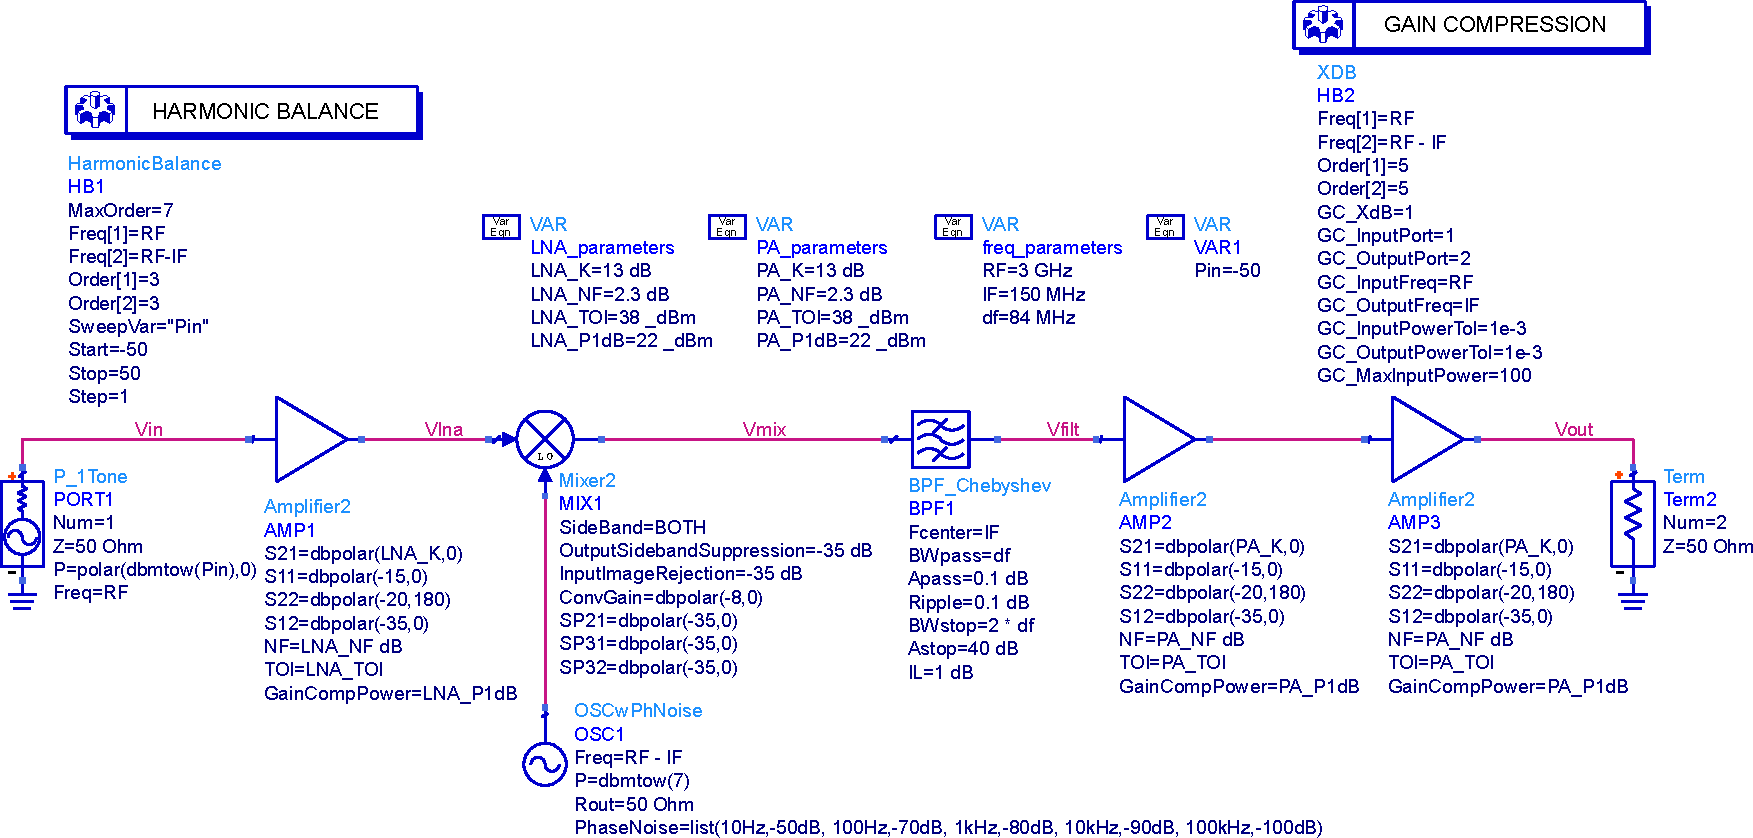
\includegraphics[width=0.8\textwidth]{simulation_modeling_schematic_2.pdf}
    \caption{Моделируемая схема}%
    \label{fig:simulation_modeling_schematic_2}
\end{figure}

\begin{figure}[!ht]
    \centering
    \begin{subfigure}[b]{0.3\textwidth}
        \centering
        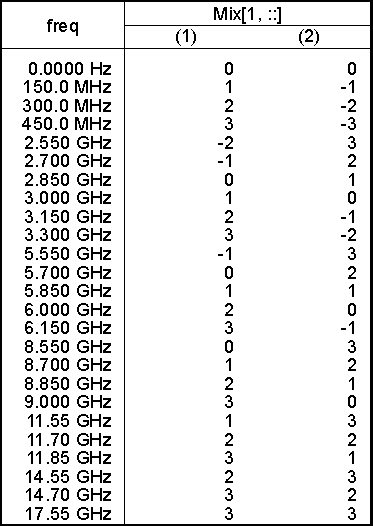
\includegraphics[width=\textwidth]{simulation_modeling_data_2_table.pdf}
        \caption{}%
        \label{fig:simulation_modeling_data_2_table}
    \end{subfigure}
    \hfill
    \begin{subfigure}[b]{0.6\textwidth}
        \centering
        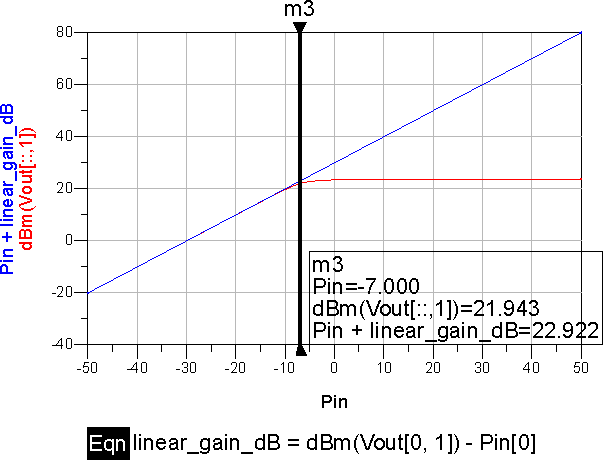
\includegraphics[width=\textwidth]{simulation_modeling_data_2_plot.pdf}
        \caption{}%
        \label{fig:simulation_modeling_data_2_plot}
    \end{subfigure}
    \caption{%
        (а) Таблица гармоник;
        (б) зависимость мощности на узле $V_{out}$ от $P_{in}$
    }%
    \label{fig:simulation_modeling_data_2}
\end{figure}

\subsection{Определение интермодуляционных искажений третьего порядка}

Отредактируем схему (Рис.~\ref{fig:simulation_modeling_schematic_3}) и запустим моделирование.
В окне результатов расчёта выведем гармоническое представление выходного сигнала (Рис.~\ref{fig:simulation_modeling_data_3_harmonics}).

\begin{figure}[!ht]
    \centering
    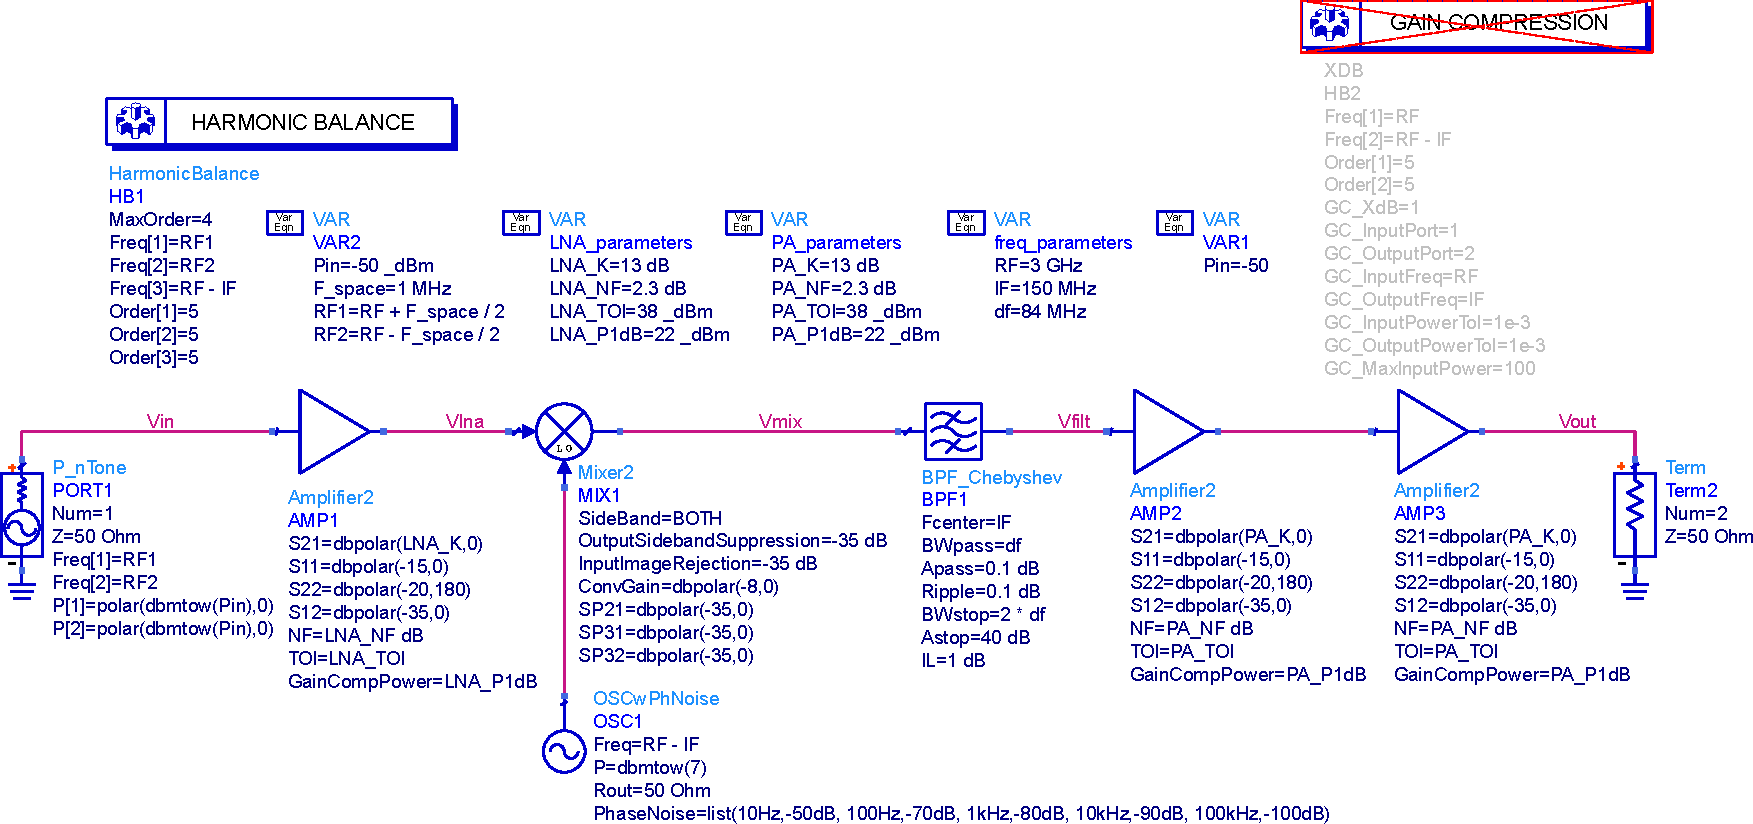
\includegraphics[width=\textwidth]{simulation_modeling_schematic_3.pdf}
    \caption{Моделируемая схема}%
    \label{fig:simulation_modeling_schematic_3}
\end{figure}

\begin{figure}[!ht]
    \centering
    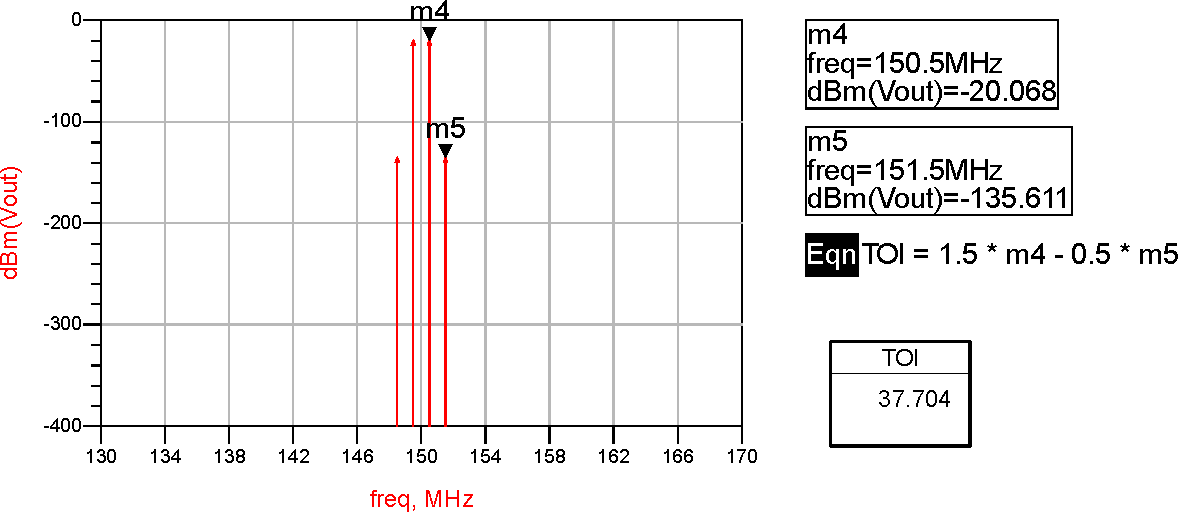
\includegraphics[width=0.7\textwidth]{simulation_modeling_data_3_harmonics.pdf}
    \caption{Гармоническое представление сигнала}%
    \label{fig:simulation_modeling_data_3_harmonics}
\end{figure}

\subsection{Анализ бюджета канала}

С помощью контроллера \elementname{Budget} определим распределение энергетических, шумовых и прочих параметров вдоль канала.
Для этого поменяем схему и настроим блок \elementname{Budget} в соответствии с Рис.~\ref{fig:simulation_modeling_schematic_4}.

\begin{figure}[!ht]
    \centering
    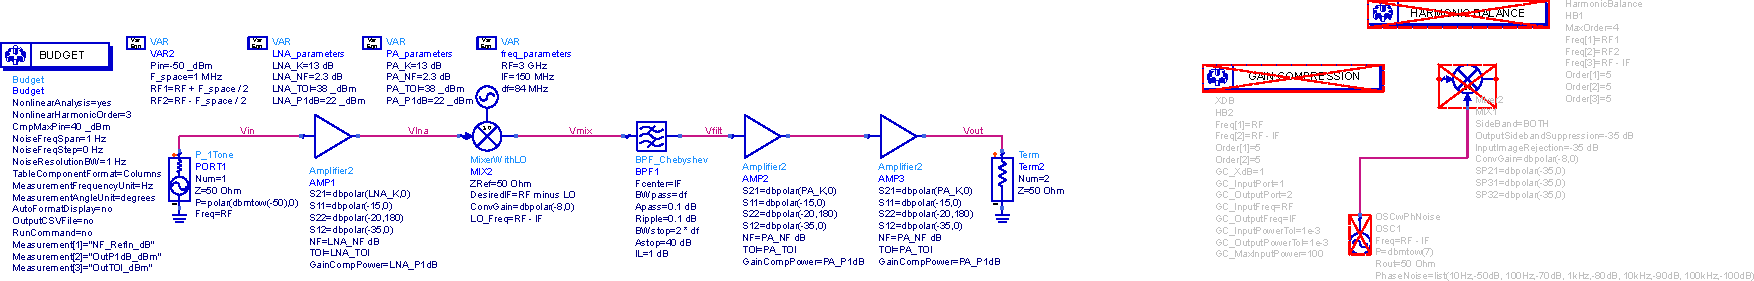
\includegraphics[width=\textwidth]{simulation_modeling_schematic_4.pdf}
    \caption{Моделируемая схема}%
    \label{fig:simulation_modeling_schematic_4}
\end{figure}

Промоделировав схему, выведем на экране данных таблицу (Рис.~\ref{fig:simulation_modeling_data_4_budget_table}).

\begin{figure}[!ht]
    \centering
    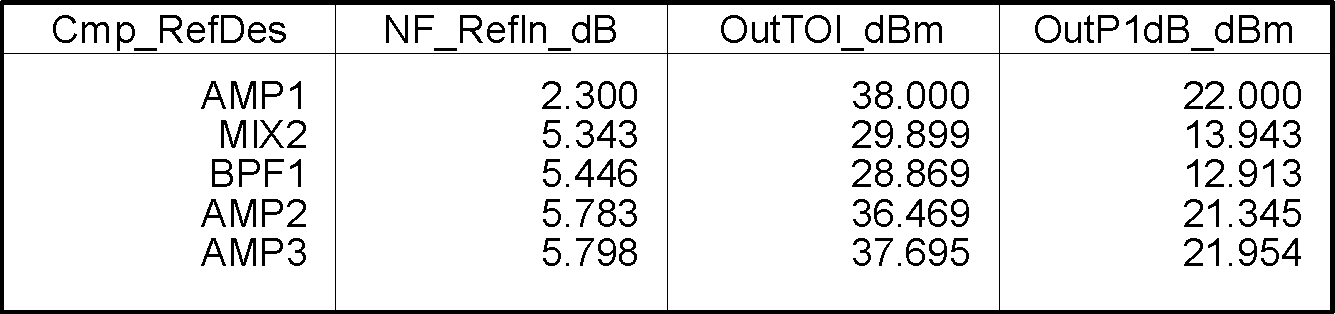
\includegraphics[width=0.7\textwidth]{simulation_modeling_data_4_budget_table.pdf}
    \caption{Бюджет канала}%
    \label{fig:simulation_modeling_data_4_budget_table}
\end{figure}

\subsection{Анализ фазовых шумов}

Проведём анализ фазовых шумов.
Для этого воспользуемся блоком \elementname{NoiseCon}.
Изменим схему и настроим этот блок в соответствии с Рис.~\ref{fig:simulation_modeling_schematic_5}.

\begin{figure}[!ht]
    \centering
    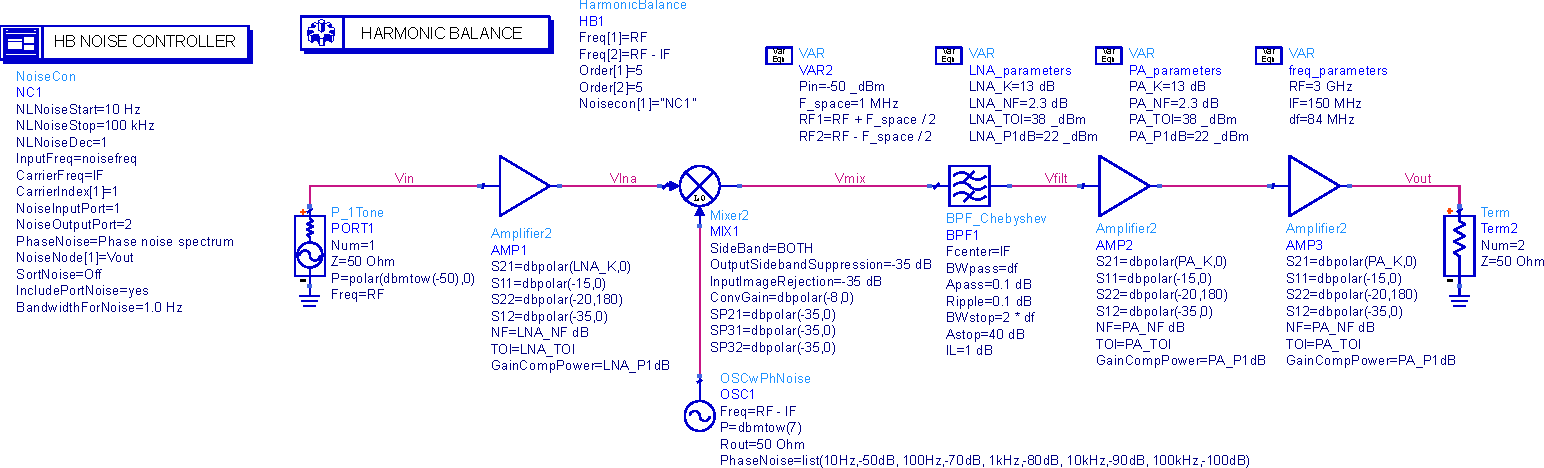
\includegraphics[width=\textwidth]{simulation_modeling_schematic_5.pdf}
    \caption{Моделируемая схема}%
    \label{fig:simulation_modeling_schematic_5}
\end{figure}

Запустим моделировани и добавим прямоугольный график зависимости $pnmx$ от $noisefreq$.
Последнюю для удобства выведем в логарифмическом масштабе.

\begin{figure}[!ht]
    \centering
    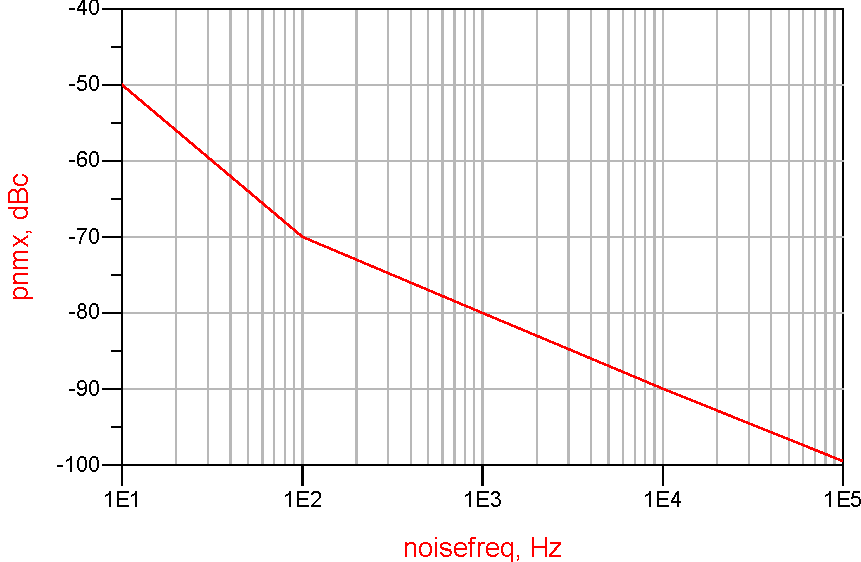
\includegraphics[width=0.7\textwidth]{simulation_modeling_data_5_phase_noise.pdf}
    \caption{Анализ фазовых шумов}%
    \label{fig:simulation_modeling_data_5_phase_noise}
\end{figure}
